\documentclass[../Cryptography.tex]{subfiles}

\begin{document}
\chapter{Historical ciphers and general principles}
Cryptology is a term merging two similar fields of stuy : cryptograph and cryptanalysis.
\begin{itemize}
    \item \term{Cryptography} : the study of secret writing with the goal of \textbf{hiding a message}.
    \item \term{Cryptanalysis} : breaking cryptosystems. 
\end{itemize}
\section{Cryptography}
In cryptography, to hide a message, there are two things that interest us : hide our content (\term{Confidentiality}) and authenticating a message (\term{Authentication}).

\subsection{Confidentiality}
For a generic cryptosystem that ensures confidentiality of a message, we talk about two operations : 
\begin{itemize}
    \item \term{Encryption} of a plain-text \green{message} to get a \rouge{ciphertext}
    \item \term{Decryption} of a \rouge{ciphertext} to retrieve a \green{message}
\end{itemize}

We always have to picture two persons communicating with each other, and eventually a third-party intervenant trying to have access to the conversation. Hence, encryption and decryption are meaningless without talking about the intervenants, that we choose to name Ali and Bachar \footnote{Instead of Alice and Bob, let's change continent a bit.}. \\

Ali and Bachar's communicating schema is the following : the first encrypts a message, sends it to the seconds that knows how to decrypt it to find the original content of the message. As they must be the only ones able to encrypt and decrypt the same way, they must have some kind of \term{key}.\\

This key generation/sharing/storage is the source of the division of cryptograph in two kinds : a symmetric way or an asymmetric way.
\begin{itemize}
    \item In \term{Symmetric crypto}, also called \term{secret-key} crypto, both parts have an encryption and a decryption method, and they \textbf{share the same key that is secret}, kepts out of the sight of any outsider. We also assume that the encryption and decryption algorithms are \textbf{publicly known}.
    \item In \term{Asymmetric crypto} (since 1976), the two possess both a private and a public key. They share their public key, but never their private key ! \\ 
\end{itemize}

So in general, we will talk about encryption as a mechanism that takes a message $m$, encrypts it with a key $k_E$ to get a ciphertext $c$, and sends it. As for decryption, it takes a ciphertext $c$, decyrpts it under a key $k_D$ to obtain $m$. 
\begin{itemize}
    \item Symmetric : $k_E = k_D$
    \item Asymmetric : $k_E$ is public, $k_D$ is private.
\end{itemize}

\subsection{Authentication}
As for authentication, we \textbf{are not trying to hide anything}. The message is sent in full plain-text from Ali to Bachar. Our goal here is to \textbf{check} the source of our message, assure its authenticity.\\

Similarly to encryption/decryption, we here have two mechanisms with keys :
\begin{itemize}
    \item Authentication : Ali generates a tag under a key $k_A$, and sends the couple $(m,\mathrm{tag})$ to Bachar
    $$m \Rightarrow (m, \mathrm{tag})$$
    \item Verification : Bachar receives $(m,\mathrm{tag})$, and under key $k_V$, identifies the source.
    $$(m, \mathrm{tag}) \Rightarrow \{m, \perp\}$$
\end{itemize}

In symmetric crypto, $k_A = k_V$ and is \textbf{secret}. In this case, the tag is more commonly called \term{Message Authentication Code} (MAC). \\

In asymmetric crypto, $k_A$ is private and $k_V$ is public. In this case, the tag is called "\term{signature}".
To do so, with the message, Ali sends a tag. \\

\begin{center}
    \includegraphics[width=\linewidth, page={4}]{Slides/1-Historical-Principles.pdf}
    \includegraphics[width=\linewidth, page={5}]{Slides/1-Historical-Principles.pdf}
\end{center}

\section{Cryptanalysis}
Cryptanalysis is the field that studies algorithms and ways of breaking a cryptosystem. This means, recovering the message, or recovering the key. There are several ways to do this, going from "little average mathematician boi that exploits the inner structure of the scheme" to the "chad asking you your password with a gun pointing to the head". All the methods, from the first to the last, are part of \textbf{cryptanalysis}. But in this course, we focus on what we call \textbf{mathematical cryptanalysis}. We will also place ourselves in the Kerckhoff's principles.\\

\bg{Kerckhoff's principles for cryptographic systems}{
The security of a cryptosystem must only rely on the \textbf{secrecy of its key}. We hence assume, when evaluating the security of a system, that everything is known : length of the messages, encryption and decryption scheme.
}

\subsection{Mathematical cryptanalysis}

\bg{Some definitions}{
    \begin{itemize}[label=\tiny $\blacksquare$]
        \item Key space : set of all possible keys
        \item Brute-force attack : attack that tries all the keys of the key space.
    \end{itemize}
}
This branch studies brute-force attacks and analytical attacks. Analytical attacks can be of several types : exploiting some statistical patterns, length extension attack, ... \\

\subsection{Key length}
This is an informative section on key length, just to develop an intuition on the impact of the length of a key in a cryptographic system. \\

First, it is important to mention that the key length in a \textbf{symmetric} crypto system is relevant only if the brute-force attack is the best-known attack. \\

Excluding this case, then the guaranteed security of a cryptosystem according in function with the key length is very different depending on the kind of crypto : a 80-bit key in symmetric crypto can ensure the same security as a 1024-bits key asymmetric scheme (such as RSA).

\subsection{Time to break}
Here is an indicator of the meaning of the "time-to-break" (TTB) of cryptosystems in function of the key length for a \textbf{symmetric scheme}.
\begin{figure}[h]
    \centering
    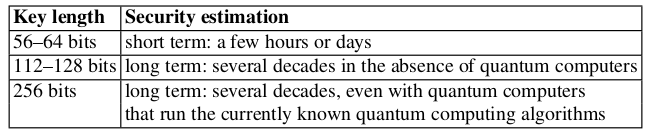
\includegraphics[width=0.7\linewidth]{images/1-TTB.png}
\end{figure}
\section{Some ciphers}
\subsection{Shift encryption scheme}
Chose a key $k$ between $0$ and $26$, message $m$ also between $0$ and $26$. The shift encryption scheme is all about XORing the message with the key :
$$
\begin{array}{lll}
    E_k(m) &= m + k \mod{26} &= c \\
    D_k(c) &= c - k \mod{26} &= m
\end{array}$$
It is really dumb : as the key space is very limited ($26$), it is quickly subject to brute-force methods.
\subsection{Mono-alphabetic substitution}
The mono-alphabetic cipher consists in replacing each letter of the message by a corresponding letter in a mixed alphabet chosen randomly. So we define a substitution table, and we apply our mapping. Let's break it down a little bit.
\begin{itemize}
    \item It is a symmetric scheme.
    \item The key space is $s = 26! > 4\cdot 10 ^{26}$ : a brute-force attack would take some time.
    \item It is breakable using a statistical approach.
\end{itemize}
\begin{center}
    \includegraphics[page=10, width=0.49\textwidth]{Slides/1-Historical-Principles.pdf}
    \includegraphics[page=11, width=0.49\textwidth]{Slides/1-Historical-Principles.pdf}
\end{center}

\subsection{Poly-alphabetic substitution}
Instead of encrypting a entire message with the same mapping, we here divide the message into $t$ blocks.
$$ x = x_1 \Vert x_2 \Vert \dots \Vert x_t$$
Then, we define a mapping for each block. This will be encoded in the key $k$ of the scheme. Indeed, each $k\in K$ will define a \textbf{set of permutations} 
$$k \Rightarrow (p_1, p_2, \dots, p_t) \; .$$
Hence, $E_k(x)$ will be given by 
$$E_k(x) = p_1(x_1) \Vert p_2(x_2) \Vert \dots \Vert p_t(x_t) \Vert $$

As for the decryption key $k'$, it needs to define the set of the $t$ corresponding inverse permutations :

$$k' \Rightarrow (p_1^{-1}, p_2^{-1}, \dots, p_t^{-1}) \; .$$

\subsection{Vigenère cipher} 
\begin{itemize}
    \item Message $m$ of length $|m|$, chosen in $(\mathbb{Z}_{26})^\star$
    \item Key space $K \subset (\mathbb{Z}_{26})^t$. Size : logically $26^t$
    \item Key $k$ taken randomly in $K$, so 
    $$k = (k_0, k_1, \dots, k_{t-1}) \in K$$
\end{itemize}
Then, the encryption of $m$ will result in the concatenation of the XORing of each bit $m_i$ with a part of the key that. Remember that the key has only $t$ parts, so we will repeat the same parts if the message is very long ! The same with a modular difference for the decryption

$$\begin{array}{rll}
    E_k(m) \equiv E_k(m_0 \Vert m_1 \Vert \dots \Vert m_{|m|-1}) &=  \underset{\scriptscriptstyle{0\leq i \leq |m|-1}}{\Vert} (m_i + k_{i  \mod{t}}) &= c \\
    D_k(c) \equiv E_k(c_0 \Vert c_1 \Vert \dots \Vert c_{|c|-1}) &=  \underset{\scriptscriptstyle{0\leq i \leq |c|-1}}{\Vert} (c_i - k_{i  \mod{t}}) &= m \\
\end{array}$$

In practice, the key can actually be a $t$-long string. During the process, each character is converted to a number.

\begin{center}
    \includegraphics[width=0.8\linewidth, page=15]{Slides/1-Historical-Principles.pdf}
\end{center}

\subsubsection{Cryptanalysis of Vigenère cipher}
We stick to Kerckhoff's principles : so we know how every message is encrypted, and the only thing that is kept secret is the key $k$. We don't even know its length $t$. And as it has been seen before, some bits of $m$ are encoded with the same key chunk because of the modulo in the XOR ($k_{i\mod t})$. So we can group the bits of $m$ that are encoded with the same chunks.

$$m_i, m_{i+ t}, m_{i+2t} \longleftarrow k_{i\mod t}$$

For each chunk, we see that we actually have a simple shift encryption scheme that can be easily broken. So, if we know the length $t$ of the key, we can break Vigenère cipher easily. \\

How to find the length of the key ? We can try brute-force. It will work. But there is a better method, using the \textbf{index of coincidence}. \\

Now that we have introduced the fundamental ciphers, we can move on some more cryptanalysis definitions : how do we quantify the security of cryptosystems ?


\section{Perfect secrecy (PS -- unconditional security)}
A first definition that comes into the hand when talking about security of cryptosystems is \textbf{perfect secrecy}. It is an \textbf{ideal property} that a cryptosystem can achieve. In English, it states that it must not leak any information, even to an adversary with unlimited computational power. In mathematical terms (not real mathematics, but mmmhh), it states the following 
\bg{Perfect secrecy}{
    An encryption scheme satisfies perfect secrecy an adversary can not distinguish two random encryptions : 
    \begin{itemize}
        \item For any two messages $m_1, m_2 \in M$
        \item For every ciphertext $c \in C$
        \item Choosing a key $k \in K$
    \end{itemize}
    $$\mathrm{Pr}\left[\mathrm{Enc}_k(m_1) = c\right] = \mathrm{Pr}\left[\mathrm{Enc}_k(m_2) = c\right]$$
}
\subsection{Perfect secrecy and length of keys}
Claude Shannon showed that for a system to achieve perfect secrecy, the length of the key must be at least the length of the message. Note that it is possible to have a scheme with a key much longer than the message but for it to be not secure at all... It is an implication : it must, but it is not sufficient.  \\
\begin{center}
    \includegraphics[width=\linewidth, page=27]{Slides/1-Historical-Principles.pdf}
\end{center}
Note that in practical, this is a property that annoys us a lot because for long messages, we must have a longer key. We will see later some \textit{lighter} security definitions.

\subsection{One-time pad (OTP)}
The one-time pad encryption scheme is quite easy : it is close to the Vigenère cipher, except for the fact that \textbf{the key is as long as the message}. It can thus ensure PS. But, does it really ? \\

We are given a message space $$ M = (\mathbb{Z}_2)^t$$ and $C = K = M$. This means we play with binary strings. The key will be written as $$ k = (k_0,k_1, \dots, k_{t-1}) \; ,$$
and the messages, ciphertexts, can also be similarly written. The scheme is the following :
$$
\begin{array}{lll}
    E_k(m) \equiv E_k(m_0, m_1, \dots, m_{t-1}) &= (m_i + k_i)_{0\leq i \leq t-1} &= c \\
    D_k(c) \equiv D_k(c_0, c_1, \dots, c_{t-1}) &= (c_i - k_i)_{0\leq i \leq t-1} &= m \\
\end{array}$$
It looks indeed similar to the Vigenère cipher. But here, let's compute the probability of knowing a plaintext -- ciphertext pair.


\begin{align*}
\mathrm{Pr}[E_k(m) = c] &= \mathrm{Pr}[m\oplus k = c] && \text{Bit-wise operator}\\
&= \mathrm{Pr}[k = m \oplus c] && \text{Because $m\oplus m = 0$}\\
&= 2^{-t} && \text{Because $k$ is chosen randomly in $(\mathbb{Z}_2)^t$}
\end{align*}

We thus prove that the OTP achieves perfect secrecy. It may look like Vigenère's, but in security ways, it is way different. OTP is the ideal scheme, Vigenère's is easily broken as we saw. \\

Why "one-time" pad ? Because if we use twice the same key for a different message, there is information that is leaked from the system. In particular, we can find a link between the ciphertexts and the messages. Indeed :
\begin{align*}
    \text{If} &&& c_1 = m_1 \oplus k \\
    \text{and} &&& c_2 = m_2 \oplus k \\
    \text{Then} &&& c_1 \oplus c_2 = m_1\oplus m_2 && \text{Because $k\oplus k = 0$} \\
\end{align*}

\section{Computational security}
As we already saw, perfect secrecy requires the key being at least as long as the message. This annoys us very much. Some systems can be very secure \textbf{without achieveing perfect secrecy}. This allows us to leak some information. This introduces us the notion of \textbf{computational security}. \\


\begin{center}
    \includegraphics[width= \linewidth, page=37]{Slides/1-Historical-Principles.pdf}
\end{center}

We really need to interpret this with the example : if the key space of a system is of size $2^{128}$ and that for the best attack, the probability of finding $k$ after $t$ attempts is $\varepsilon(t) = t/2^{128}$, then the scheme is $s=128$-bit secure. 

\section{Security principles}
There is a big gap between cryptography and practical cryptosystems. In practical, none of the cryptosystems will see offer perfect secrecy. The only ways to gain confidence in the security of a scheme is by \textit{peer-reviewing}. Particularly, the \textbf{algorithm must be public}, first for people to help proving its security/breaking it, but most importantly to stick to Kerckhoff's principles.
\subsection{Goals of an adversary}
\includegraphics[width=0.8\linewidth, page=45]{Slides/1-Historical-Principles.pdf} 

\subsection{Ability to query the scheme}
\includegraphics[width=0.8\linewidth, page=47]{Slides/1-Historical-Principles.pdf} 

\subsection{Taxonomy of attacks}
\includegraphics[width=0.8\linewidth, page=49]{Slides/1-Historical-Principles.pdf}

\subsection{Formal definition of an encryption scheme}
\includegraphics[width=0.8\linewidth, page=50]{Slides/1-Historical-Principles.pdf} 

\subsection{Semantic security}
An encryption scheme is \textbf{semantically secure} if : when the adversary can compute  with the ciphertext something about the plaintext in a polynomial time, it can also do it without the ciphertext (in a polynomial time). \\

This immediately implies that \textbf{deterministic encryption} is not semantically secure. To make it secure, we must go \textbf{probabilistic}. Using a nonce for the key generation.

\bg{Nonce}{
    A \textit{nonce} is a number used once. Most likely randomly generated.
}

\subsection{INDististinguishability games}
Let's play a bit, and introduce the following game. It is called the "IND-game", and we apply it on an encryption scheme $\mathcal{E} = (\mathrm{Gen}, \mathrm{Enc}, \mathrm{Dec})$. If the adversary can not win it with other than with a negligeable advantage against a \textbf{random guess}, we are good. \\

Basically, it ensures that an adversary can not know between two plaintexts, even if they are chosen, which of them was encrypted, if it is given a ciphertext. This game can be twisted and allow the adversary to query the encryption function giving us the IND-CPA game (includes steps \ref{enum:cpa1} and \ref{enum:cpa2})

\bg{IND(-CPA/CCA) game}{
    \begin{enumerate}
        \item Challenger generates a key $k \longleftarrow \mathrm{Gen}()$.
        \item \label{enum:cpa1}
        [CPA/CCA only] \rouge{Adversary queries $\mathrm{Enc}_k$ with plaintexts of his choice} 

        [CCA only] \green{and $\mathrm{Dec}_k$ with ciphertexts of his choice}
        \item Adversary chooses two same-length plaintexts $m_1, m_2 \in M \wedge |m_1| = |m_2|$ and gives them to the Challenger.
        \item Challenger randomly encrypts $m_1$ or $m_2$, gives the ciphertext $c_x = E_k(m_x)$ to the adversary.
        \item \label{enum:cpa2} 
        [CPA/CCA only] \rouge{Adversary queries $\mathrm{Enc}_k$ with plaintexts of his choice} 
        
        [CCA only] \green{and $\mathrm{Dec}_k$ with ciphertexts of his choice}
        \item Adv. guesses $x'$ was encrypted
        \item Adv. wins if $x = x'$
    \end{enumerate}
}
We note the "Advantage" of a system the probability that this winning situation is far from $1/2$, that corresponds to a totally random guess. Formally :
$$\mathrm{Advantage} \equiv \varepsilon = \left| \mathrm{Pr}[\mathrm{win}] - \frac{1}{2}\right| \; .$$

\bg{Note}{
    For symmetric crypto, the IND game only addresses the security of a single encryption. Indeed, it needs the challenger to encrypt, as there is no public key \footnote{This semantically makes sense but I don't even understand what we should conclude of this.}. The game can only be played \textbf{online}.
}

\subsection{Extending security strength definition}
Hence, we can extend the security strength definitions for indististinguishability. 

A system id $(t,d,\varepsilon)-$IND-CPA (resp. IND-CCA) secure if any adversary running at most $t$ attempts and having access to $d$ data succeeds in winning the respective game with Advantage at most $\varepsilon$. \\

Here, we mentioned a limit quantity $d$ of data that we authorize the adversary to query with. But what attempts are we counting ? If we are in asymmetric crypto, then the encryption key is completely public so anyway the adversary can compute any encryption he wants. The decryption key is however private, so $d$ in asymmetric crypto refers to the number of times an adversary can query the decryption scheme, and is hence logic to be found only in the IND-CCA game. Similarly for the symmetric case : here $d$ refers to both encryption and decryption querying because both rely on a secret key. This gives us the table on the slide below : 

\begin{center}
    \includegraphics[width=0.8\linewidth, page=59]{Slides/1-Historical-Principles.pdf}
\end{center}

\subsection{INDististinguishability using a diversifier (nonce)}
In symmetric crypto, encryption is diversified at each use : encryption takes an extra parameter $d$ randomly-chosen, completely public. The decryption also takes $d$ as input. \\

Thus, the symmetric-key encryption scheme must be modified :
\begin{center}
    \includegraphics[width=0.8\linewidth, page=61]{Slides/1-Historical-Principles.pdf}
\end{center}

Here is the IND-CPA game with a diversifier :
\bg{IND-CPDA game (chosen plaintext and diversifier)}{
    \begin{enumerate}
        \item Challenger generates a key $k \longleftarrow \mathrm{Gen}()$.
        \item \label{cpda:nonce1} Adversary queries $\mathrm{Enc}_k$ with $(d,m)$ of his choice.
        
        \item \label{cpda:nonce2} Adversary \rouge{chooses $d$} and $m_1, m_2$ and gives them to the Challenger.
        \item Challenger randomly encrypts $m_1$ or $m_2$, gives the ciphertext $c_x = E_k(d, m_x)$ to the adversary.
        \item \label{cpda:nonce3} Adversary queries $\mathrm{Enc}_k$ with $(d,m)$ of his choice
        \item Adv. guesses $x'$ was encrypted
        \item Adv. wins if $x = x'$
    \end{enumerate}
}
But \textbf{attention} : the adversary \textbf{must} respect that $d$ is a \textbf{nonce} !! The nonces used at steps \ref{cpda:nonce1}, \ref{cpda:nonce2}, and \ref{cpda:nonce3} \textbf{must all be different}.

\section{Authentication schemes}
What about authentication schemes ? Recall that our goal here is not to hide a message : the message is sent in plain text. Here, we want to provide a signature of our message, and to recognize someone's signature. So the adversary has the following goals :
\begin{itemize}
    \item Recover the (secret or private) key
    \item Forgery : be able to send a message that does not come from an authentic party and is still verified
    \item Find a property that distinguishes the scheme from ideal.
\end{itemize}

And he is allowed to get :
\begin{itemize}
    \item Known messages and corresponding tags 
    \item Chosen messages and corresponding tags
\end{itemize}

\subsection{Types of forgeries}
\begin{itemize}
    \item Universal forgery : the attack must be able to work for any message, possibly chosen by a challenger 
    \item Selective forgery : the adversary chooses the message beforehand
    \item Existantial forgery : the message content is \textbf{irrelevant}, the adversary can choose it adaptatively just to make the attack work. We guess that this is not really senseful and a weak attack.
\end{itemize}

\subsection{Taxonomy of authentication scheme attacks}
\begin{center}
    \includegraphics[width=0.8\linewidth, page=69]{Slides/1-Historical-Principles.pdf}
\end{center}

\subsection{Formal definition of an authentication scheme}
\begin{center}
    \includegraphics[width=0.8\linewidth, page=70]{Slides/1-Historical-Principles.pdf}
\end{center}

\subsection{Some games for unforgeability : EU-CMA}
\begin{center}
    \includegraphics[width=0.8\linewidth, page=71]{Slides/1-Historical-Principles.pdf}
\end{center}

\end{document}